\documentclass[11pt,a4paper]{article}
\usepackage[T1]{fontenc}
\usepackage[utf8]{inputenc}
\usepackage{libertine}
\usepackage[libertine]{newtxmath}
\usepackage[scale=0.95]{sourcesanspro}
\usepackage[margin=2.1cm,top=2.3cm,bottom=2.3cm]{geometry}
\usepackage{microtype,graphicx,booktabs,xcolor,amsmath,enumitem,multicol,array}
\usepackage[skins,raster]{tcolorbox}
\usepackage{titlesec,fancyhdr,caption,float}
\usepackage[scaled=0.88]{zi4}
\usepackage[colorlinks=true,linkcolor=accent,urlcolor=accent,citecolor=accent]{hyperref}

\definecolor{ink}{HTML}{14213D}
\definecolor{ink2}{HTML}{4A5568}
\definecolor{accent}{HTML}{8A1C5C}
\definecolor{panel}{HTML}{F2F0EA}
\definecolor{orange}{HTML}{DD6B1A}
\definecolor{blue9}{HTML}{2A78D6}
\definecolor{org12}{HTML}{C4501F}
\definecolor{grn15}{HTML}{138A60}

\titleformat{\section}{\sffamily\Large\bfseries\color{ink}}{\color{accent}\thesection}{0.6em}{}
\titleformat{\subsection}{\sffamily\large\bfseries\color{ink}}{\color{accent}\thesubsection}{0.5em}{}
\titlespacing*{\section}{0pt}{1.3em}{0.5em}
\titlespacing*{\subsection}{0pt}{1.0em}{0.35em}
\captionsetup{font={small,sf},labelfont={bf,color=accent},labelsep=period,margin=0.5cm}
\setlength{\parskip}{0.35em}
\setlength{\parindent}{0pt}
\pagestyle{fancy}\fancyhf{}
\renewcommand{\headrulewidth}{0.4pt}
\fancyhead[L]{\sffamily\small\color{ink2} IDC612 · Project P05}
\fancyhead[R]{\sffamily\small\color{ink2} Spectra of compressible convection from movie pixels}
\fancyfoot[C]{\sffamily\small\color{ink2}\thepage}
\newcommand{\Ra}[1]{$\mathrm{Ra}=10^{#1}$}

\newtcolorbox{keybox}[1][]{enhanced,colback=panel,colframe=panel,boxrule=0pt,arc=3pt,left=10pt,right=10pt,top=7pt,bottom=7pt,
  borderline west={3pt}{0pt}{accent},fontupper=\small,#1}
\newtcbox{\stat}[1][]{enhanced,colback=white,colframe=ink,boxrule=0.6pt,arc=3pt,nobeforeafter,valign=top}

\begin{document}
\thispagestyle{empty}
\begin{tcolorbox}[enhanced,colback=ink,colframe=ink,arc=4pt,left=16pt,right=16pt,top=14pt,bottom=14pt]
{\sffamily\color{orange}\small\bfseries IDC612 · MATH \& COMPUTATION USING PYTHON · PROJECT P05}\\[6pt]
{\sffamily\color{white}\fontsize{24}{28}\selectfont\bfseries Spectra of compressible convection,\\ read from movie pixels}\\[10pt]
{\sffamily\color{white!80!ink}\normalsize Suvid Goel \;·\; Abhay Tripathi \;·\; Vibhor Srivastava}\\[2pt]
{\sffamily\color{white!65!ink}\small IIT Kanpur \;·\; 14 November 2026}
\end{tcolorbox}

\begin{keybox}
\textbf{Abstract.} We were given four movies of compressible convection: a gas heated from below and cooled from above, in 2D at Rayleigh numbers $10^{9}$, $10^{12}$, $10^{15}$ and in 3D at $10^{8}$. Without any simulation output, we read temperature and density back from the colours and measured the energy spectra. A mirror trick turns the FFT in the bounded vertical direction into a sine series and gives the full 2D spectrum. The temperature spectrum follows the Obukhov--Corrsin $-5/3$ law at $\mathrm{Ra}=10^{12}$ and steepens at $10^{15}$, where low-pressure vortex cores carry 97\% of the temperature variance. The mean profile gives a $k^{-2}$ branch that a jump model predicts with no fitted constant. A time FFT reveals sound waves whose speed matches the ideal-gas value computed only from the constants printed on the movie.
\end{keybox}

\vspace{2pt}
\begin{tcbraster}[raster columns=4,raster equal height,raster column skip=6pt,
  raster every box/.style={enhanced,colback=white,colframe=ink!25,boxrule=0.6pt,arc=3pt,halign=center,left=3pt,right=3pt,top=5pt,bottom=5pt}]
\begin{tcolorbox}{\sffamily\Large\bfseries\color{org12} $-1.59$}\\[-1pt]{\sffamily\scriptsize spectral slope at $\mathrm{Ra}=10^{12}$\\ (theory $-5/3$)}\end{tcolorbox}
\begin{tcolorbox}{\sffamily\Large\bfseries\color{grn15} 97\%}\\[-1pt]{\sffamily\scriptsize of T variance in vortex\\ cores at $\mathrm{Ra}=10^{15}$}\end{tcolorbox}
\begin{tcolorbox}{\sffamily\Large\bfseries\color{ink} 0.98, 1.00}\\[-1pt]{\sffamily\scriptsize measured / predicted\\ mean-profile modes}\end{tcolorbox}
\begin{tcolorbox}{\sffamily\Large\bfseries\color{accent} 1.93--2.08}\\[-1pt]{\sffamily\scriptsize sound speed, against\\ 2.09 from the gas law}\end{tcolorbox}
\end{tcbraster}

\section{The data}
Each movie shows two panels: the temperature relative to the adiabat, $T-T_A(z)$, and the density relative to its adiabat, $\rho-\rho_A(z)$, with a colour bar for each (Fig.~\ref{fig:frame}). The gas is ideal with $\gamma=1.3$, adiabatic gradient $D=0.5$ and superadiabatic drop $\varepsilon=0.1$, all printed on the frames. The box is periodic in $x$ (width 4) and bounded by two plates in $z$ (height 1).

\begin{figure}[H]
\centering\includegraphics[width=0.93\textwidth]{../../Ra1e15_f100.png}
\caption{One frame of the $\mathrm{Ra}=10^{15}$ movie. Top: temperature; bottom: density; right: a zoomed window. Cold, light blobs near the bottom are low-pressure vortex cores.}\label{fig:frame}
\end{figure}

\begin{center}\small
\begin{tabular}{@{}lcccc@{}}
\toprule
\textbf{Movie} & \textbf{Ra} & \textbf{Panels} & \textbf{Frames} ($\Delta t=0.01$) & \textbf{Time span}\\
\midrule
2D box $4\times1$ & $10^{9}$ & $T$, $\rho$ & 1001 & 10\\
2D box $4\times1$ & $10^{12}$ & $T$, $\rho$, zoom & 1001 & 10\\
2D box $4\times1$ & $10^{15}$ & $T$, $\rho$, zoom & 201 & 2\\
3D box $4\times4\times1$ & $10^{8}$ & walls, lid, floor & 1001 & 10\\
\bottomrule
\end{tabular}\end{center}

\section{Method}
\subsection{From colours to fields}
Each pixel's colour is matched to the colour bar printed in the same frame, which gives $T-T_A$ (and $\rho-\rho_A$) at every pixel. The plates and side walls are located to $\pm0.5$ px, and the thin overlay lines (zoom box, tick marks) are masked and filled from their neighbours. As an independent check, the large-scale ratio of the temperature and density fluctuations returns the gas constants from the pixels alone (Section~\ref{sec:entropy}).

\subsection{Horizontal FFT}
The box wraps around in $x$, so a plain FFT of every row is exact. The spectrum is the average power over all rows and frames,
\[ E(k) = \big\langle\, |\hat T(k,z,t)|^2 \,\big\rangle_{z,t}, \]
where $k$ counts whole waves across the box. A power law $E\propto k^{-\alpha}$ is a straight line on log--log axes; we fit $\alpha$ by least squares.

\subsection{Vertical FFT: the mirror trick}
In $z$ the plates are walls, so an FFT would see a false jump where the hot bottom meets the cold top. We first remove the background line,
\[ \theta'(x,z) = T - (1-Dz) + \varepsilon z, \qquad \theta'(x,0)=\theta'(x,1)=0, \]
and then mirror each column above the top plate with a sign flip, $\theta'(2-z)=-\theta'(z)$. The extended column repeats with period 2 without any jump, and its FFT contains only sine waves:
\[ \theta'(x,z) = \sum_{m,n} \hat\theta(m,n)\, e^{ik_x x}\sin(n\pi z), \qquad k_x=\frac{2\pi m}{L},\quad k_z=n\pi . \]
All cosine parts vanish because the mirrored column is antisymmetric (Fig.~\ref{fig:mirror}). FFT in $x$ times the sine series in $z$ gives every 2D wave. Removing the mean profile ($m=0$) and summing the energy in rings of $K=\sqrt{k_x^2+k_z^2}$ gives the 2D spectrum $E(K)$.

\begin{figure}[t]
\centering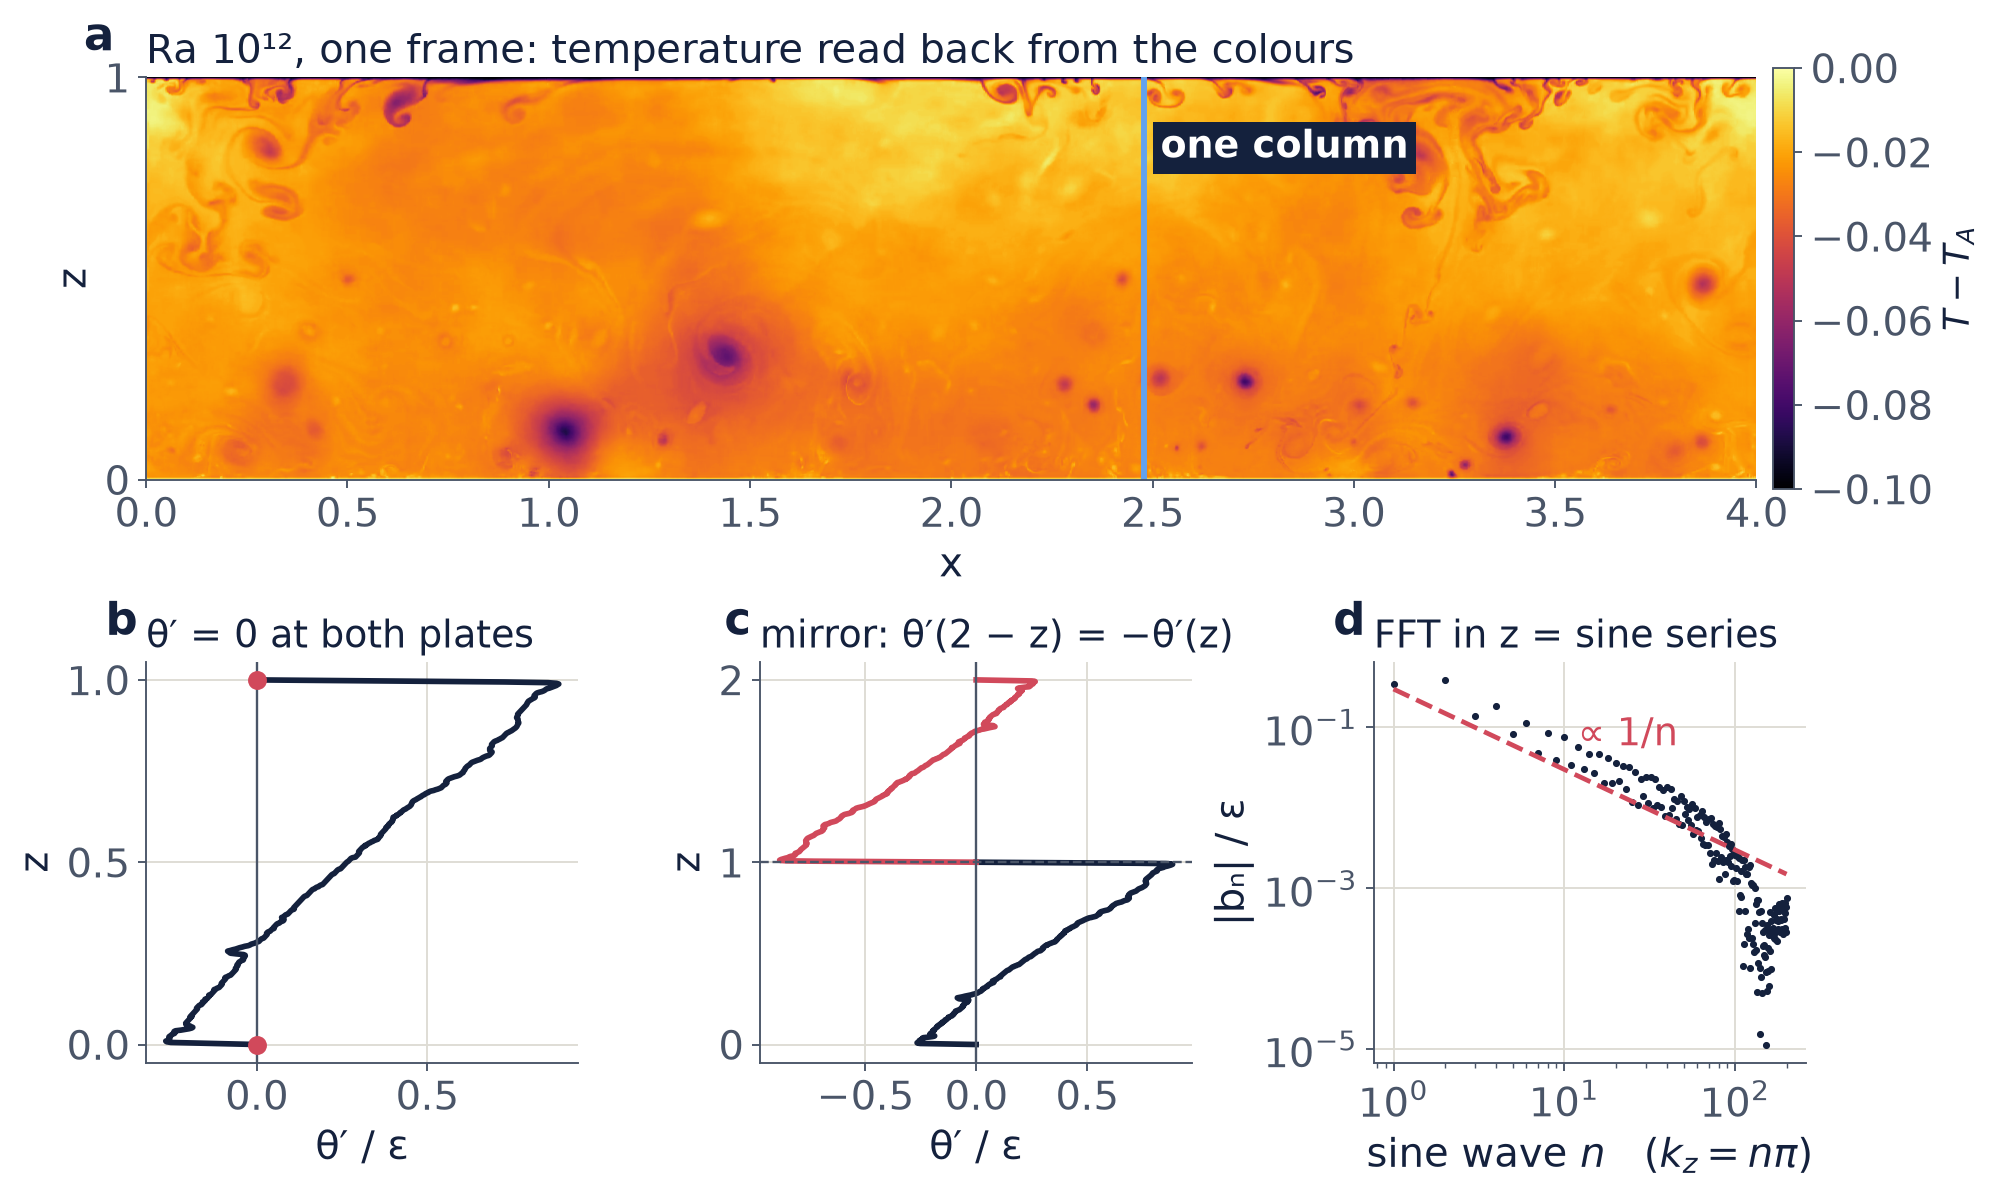
\includegraphics[width=\textwidth]{../figures/report/rep_mirror.png}
\caption{The mirror trick on real data. (a) One frame of the $\mathrm{Ra}=10^{12}$ movie. (b) One column after removing the background line: $\theta'$ is zero at both plates. (c) The column mirrored with a sign flip repeats smoothly. (d) Its FFT in $z$ is a pure sine series; the jumps at the plates make the coefficients fall like $1/n$.}\label{fig:mirror}
\end{figure}

\subsection{Error bars and validation}
Frames close in time are correlated, so 95\% intervals come from resampling blocks of frames (a moving-block bootstrap with blocks of four correlation times), or from batch means when a movie holds only a few correlation times. We validated the whole pipeline on synthetic movies drawn with the same layout, colour map and H.264 compression and with a known spectrum (Fig.~\ref{fig:valid}). At the real bitrates the 1D method returns slopes within 0.04--0.09 and the 2D method within 0.015; plate positions come back within 0.03 px, and the mean-profile amplitudes within 1\%. Only at a deliberately 3.5$\times$ lower stress-test bitrate do the high wavenumbers degrade.

\begin{figure}[H]
\centering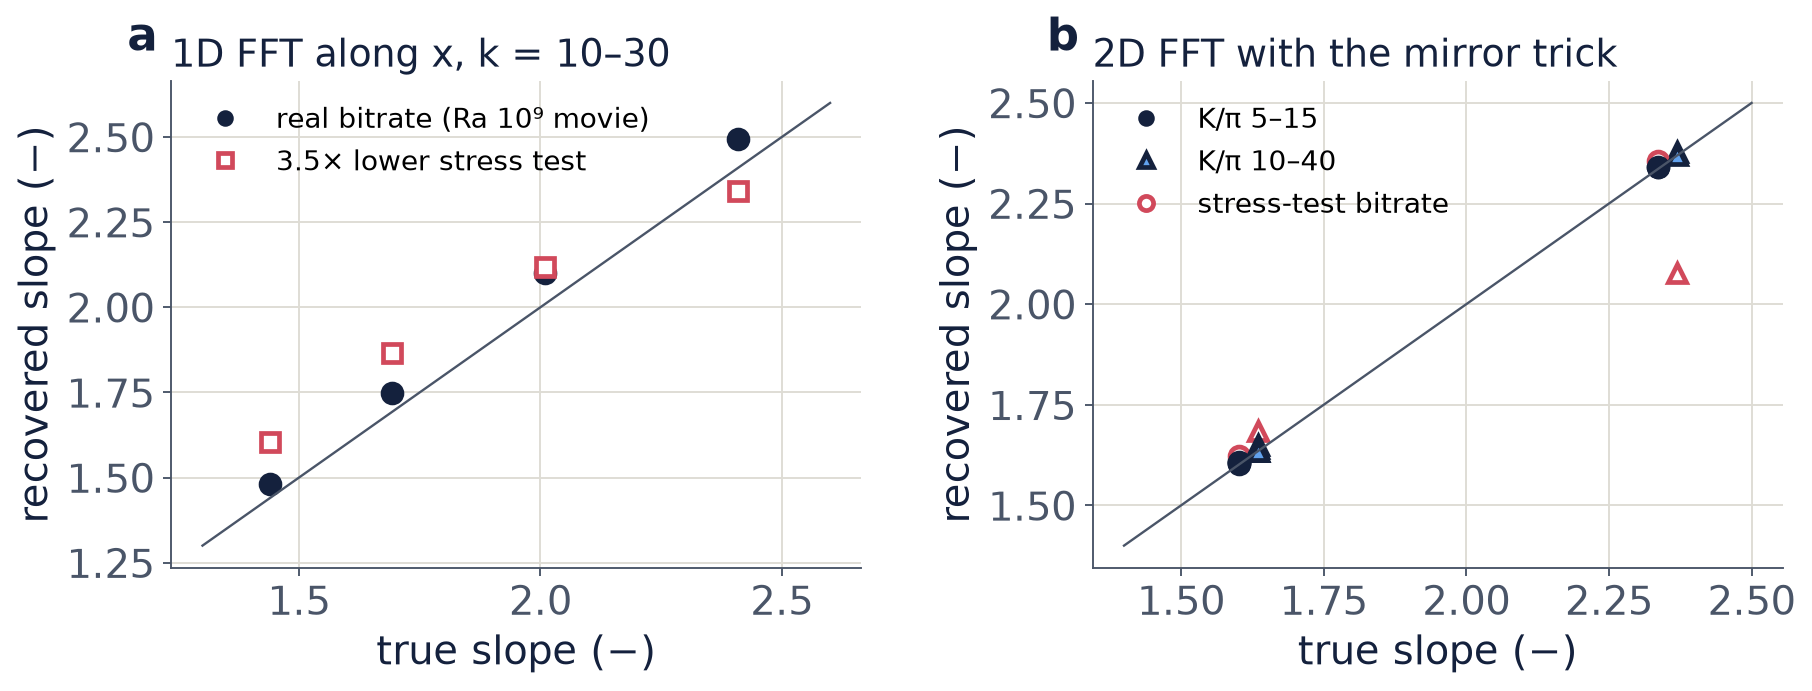
\includegraphics[width=0.86\textwidth]{../figures/report/rep_validation.png}
\caption{Validation on synthetic movies with a known slope. Points on the diagonal are perfect recovery. Filled: real bitrate; open: stress-test bitrate 3.5$\times$ lower.}\label{fig:valid}
\end{figure}

\section{Results}
\subsection{Temperature spectra}
Figure~\ref{fig:spec} shows the 1D spectra and the full 2D spectra; Table~\ref{tab:slopes} lists the slopes. At $\mathrm{Ra}=10^{12}$ both follow the Obukhov--Corrsin value $-5/3$ for a passive-like scalar. At $\mathrm{Ra}=10^{15}$ the spectrum is clearly steeper over the large scales, and at small scales both high-Ra movies approach $-2$, the value expected for sharp temperature fronts. At $\mathrm{Ra}=10^{9}$ the turbulence is weak and the straight range is short.

\begin{figure}[H]
\centering
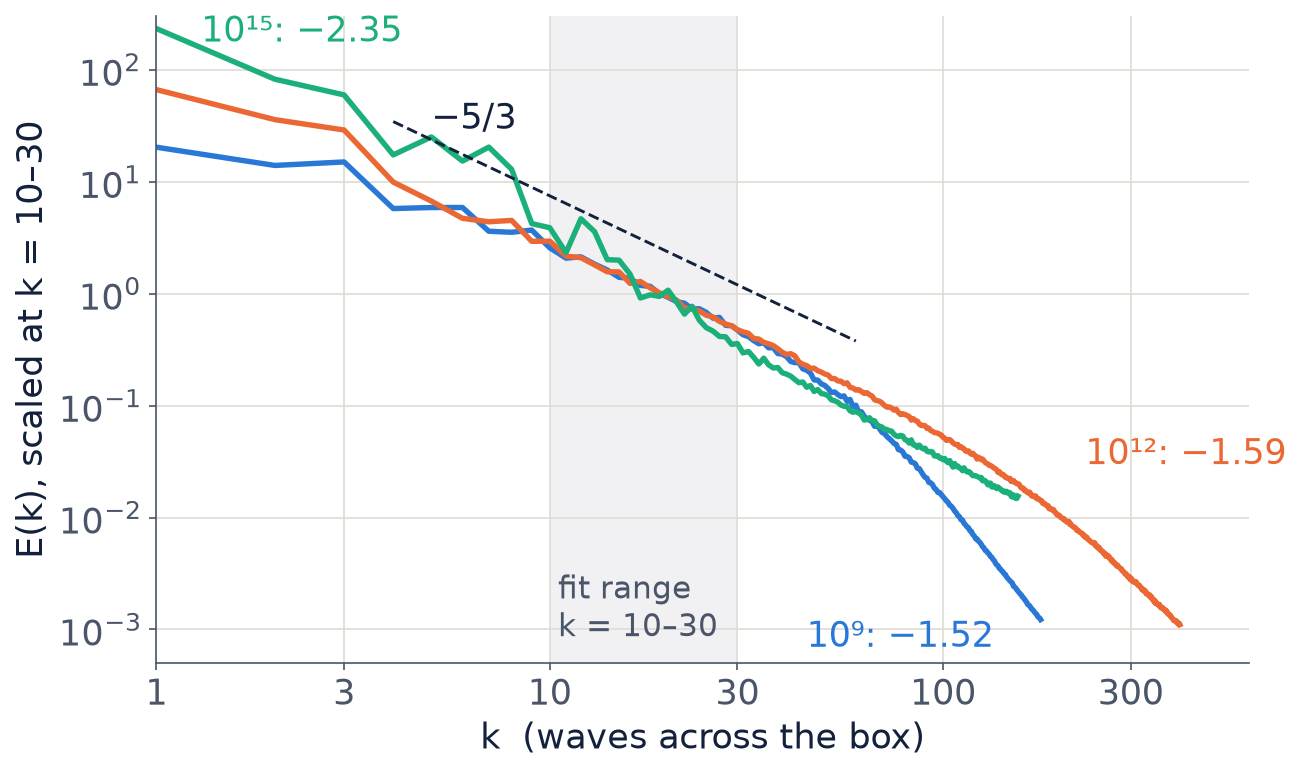
\includegraphics[width=0.77\textwidth]{../figures/report/deck_spec1d.png}\\[4pt]
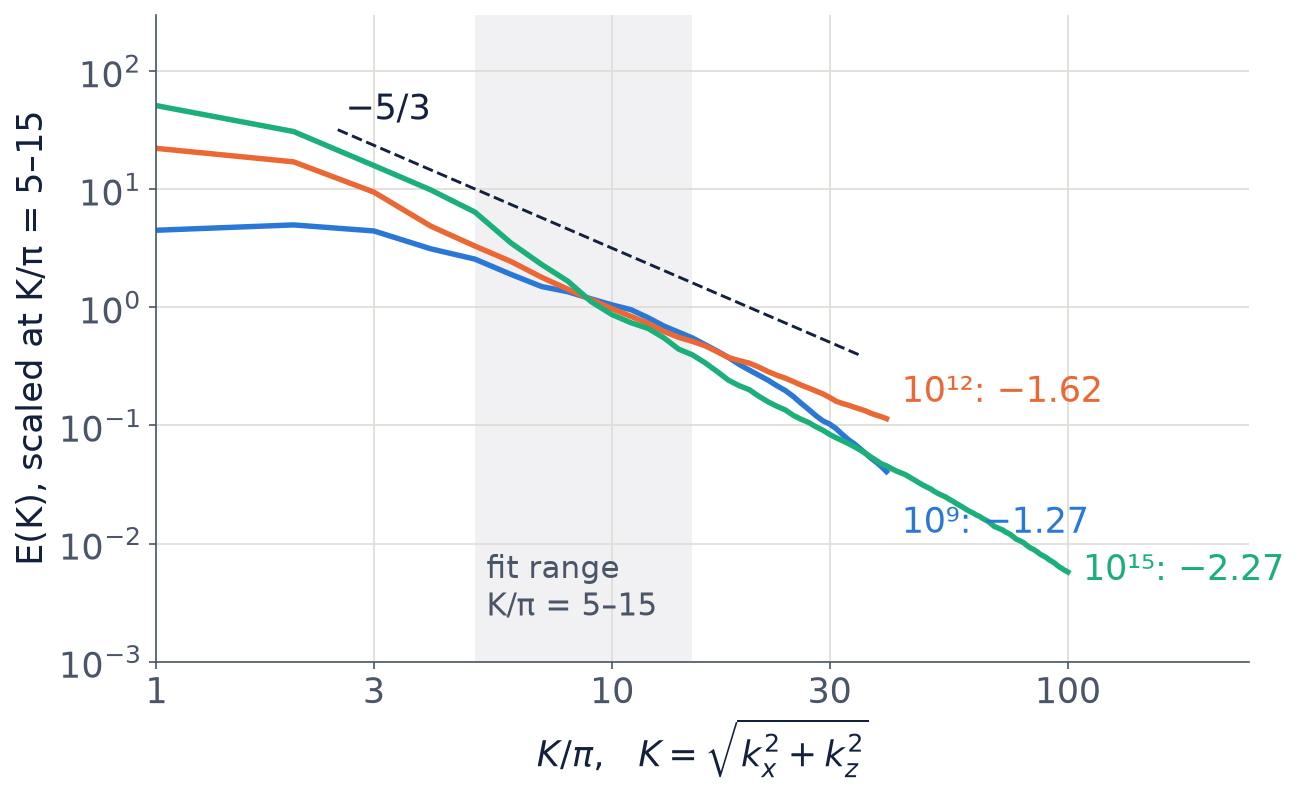
\includegraphics[width=0.77\textwidth]{../figures/report/deck_spec2d.png}
\caption{Top: 1D temperature spectra from the FFT along $x$. Bottom: full 2D spectra (FFT in $x$ $\times$ sine series in $z$), summed in rings of $K$. Dashed: slope $-5/3$; grey band: fit range.}\label{fig:spec}
\end{figure}

\begin{table}[H]\centering\small
\caption{Slopes of the temperature spectra with 95\% intervals.}\label{tab:slopes}
\begin{tabular}{@{}lccc@{}}
\toprule
 & \color{blue9}$\mathbf{Ra=10^{9}}$ & \color{org12}$\mathbf{Ra=10^{12}}$ & \color{grn15}$\mathbf{Ra=10^{15}}$\\
\midrule
1D, $k=10$--$30$ & $-1.52$ \scriptsize$[-1.65,-1.39]$ & $-1.59$ \scriptsize$[-1.69,-1.45]$ & $-2.35$ \scriptsize$[-2.42,-2.31]$\\
2D rings, $K/\pi=5$--$15$ & $-1.27$ \scriptsize$[-1.38,-1.16]$ & $-1.62$ \scriptsize$[-2.04,-1.20]$ & $-2.27$ \scriptsize$[-2.34,-2.20]$\\
Small scales & dissipation & $-1.97$ ($k$ 40--150) & $-1.92$ ($k$ 35--103)\\
\bottomrule
\end{tabular}
\end{table}

\subsection{Entropy of the spectrum and vortex cores}\label{sec:entropy}
Treating the normalised spectrum $p_k=E(k)/\sum E$ as a probability distribution, its Shannon entropy $S=-\sum_k p_k\log_2 p_k$ measures how widely the energy is spread over sizes: $S=0$ for a single mode, $S=\log_2 150=7.2$ bits for white noise. $S$ falls at every step in Ra (Fig.~\ref{fig:entropy}a), so the temperature variance sits in fewer, larger structures.

The density panel explains why. For an ideal gas $p=\rho T$, so the temperature splits exactly into an entropy part and a pressure part,
\[ \ln T = \frac{1}{\gamma}\frac{s}{c_v} + \frac{\gamma-1}{\gamma}\ln p . \]
Cold and heavy fluid is a thermal plume; cold and light fluid is a low-pressure vortex core. The pressure share of the temperature variance rises from 28\% to 77\% to 97\% (Fig.~\ref{fig:entropy}b). Vortex cores have a steep spectrum, which accounts for the steep slope at $10^{15}$. In the 3D movie the share is only 7\%: the long-lived vortices are a two-dimensional effect. The same split gives back the gas constants from the pixels: $\gamma-1=0.291$ and $D=0.475$ at $10^{12}$, $0.294$ and $0.479$ at $10^{15}$, against $0.3$ and $0.5$ printed on the frames.

\begin{figure}[H]
\centering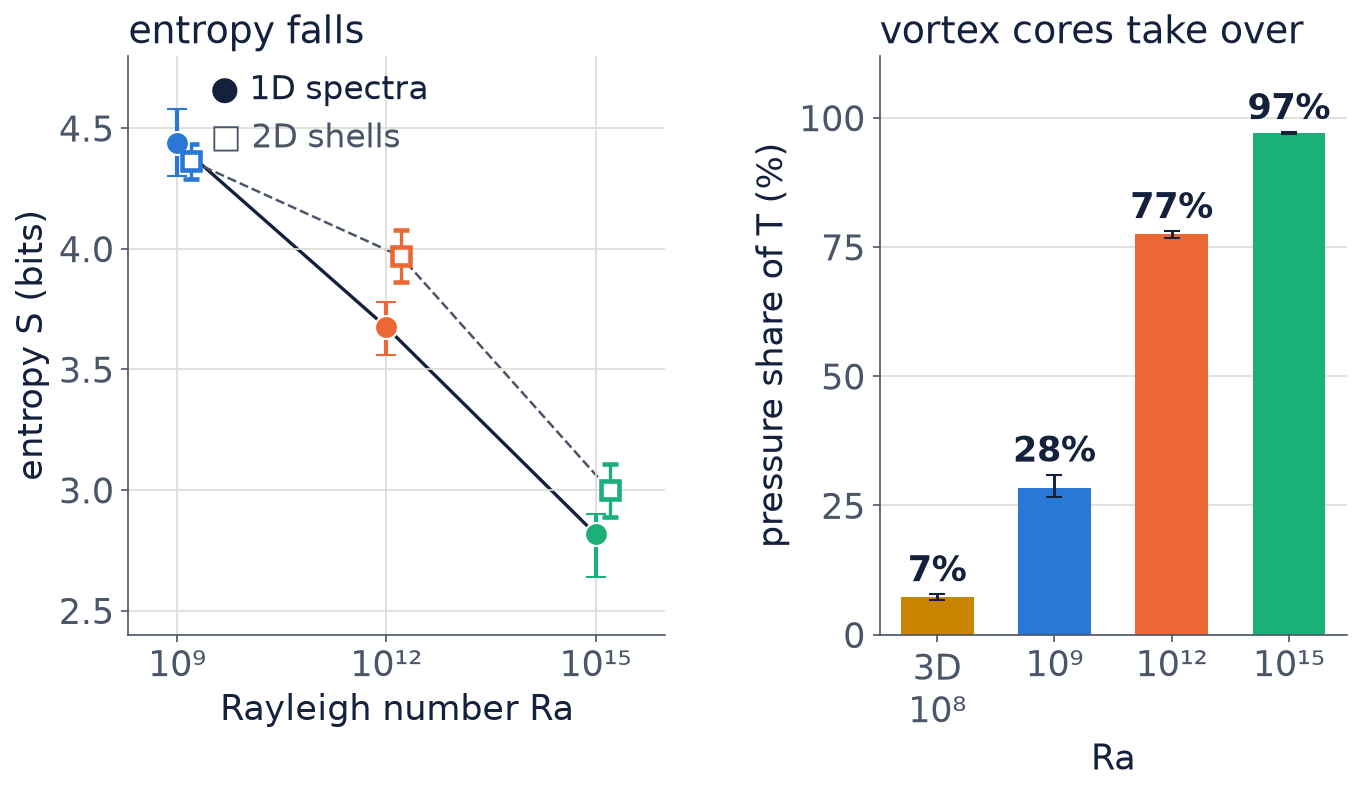
\includegraphics[width=0.82\textwidth]{../figures/report/deck_entropy.png}
\caption{(Left) Entropy of the spectrum against Ra, 1D spectra and 2D rings, with 95\% intervals. (Right) Pressure (vortex-core) share of the temperature variance; the 3D movie at $\mathrm{Ra}=10^{8}$ is shown for comparison.}\label{fig:entropy}
\end{figure}

\subsection{The mean profile and the boundary layers}
Averaging $\theta'$ over $x$ and time gives the mean profile $\Theta(z)$, which holds 96\% of the $\theta'$ variance. It is a straight line in the middle with a sharp jump at each plate (Fig.~\ref{fig:upper}, left). Writing $\Theta$ as a sine series, a jump makes the coefficients fall like $1/n$ and the energy like $n^{-2}$: the $k^{-2}$ branch of the spectrum known from studies of Rayleigh--Bénard convection \cite{verma2018}. Equal jumps are assumed there; here the gas is compressible, so we generalise to a bottom jump $J_0$ and a top jump $J_1$:
\[ \hat\Theta_n=\frac{2}{n\pi}\big[J_0-(-1)^nJ_1\big], \qquad E_n=\frac{2}{(n\pi)^2}\big[J_0-(-1)^nJ_1\big]^2 . \]
With $J_0$ and $J_1$ read directly from the profile, nothing is fitted. The measured mode amplitudes are $0.98$ and $1.00$ of the prediction at $10^{12}$ and $10^{15}$, with slopes $-2.15$ and $-2.09$. At $10^{9}$ the boundary layers are thick enough to resolve and the high modes roll off; the fitted layer thickness (0.010--0.028) agrees in size with jump divided by plate gradient (0.018--0.039). The jumps are $\approx0.25\,\varepsilon$ at the bottom and $\approx0.75\,\varepsilon$ at the top in all three movies, against $0.5$ and $0.5$ for a Boussinesq fluid: a clear signature of compressibility.

\begin{figure}[H]
\centering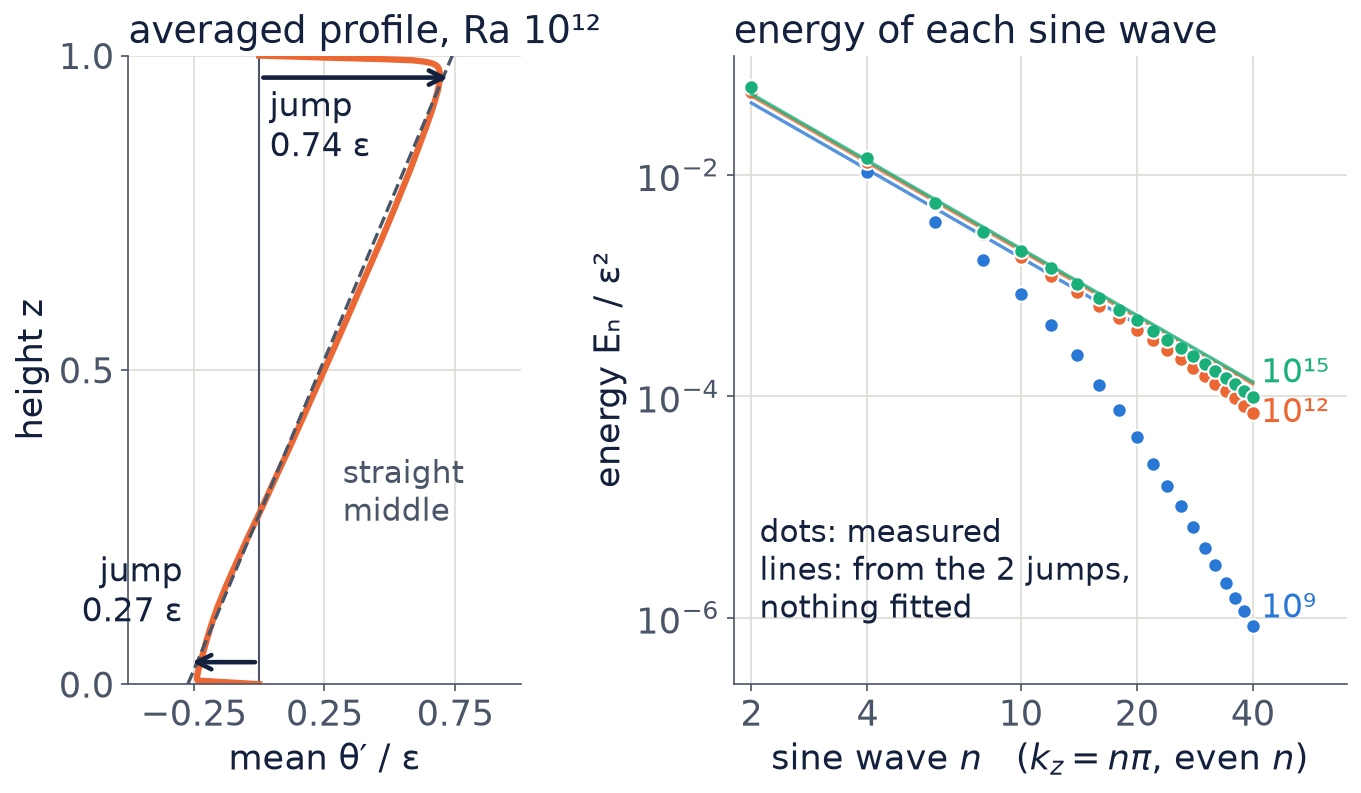
\includegraphics[width=0.85\textwidth]{../figures/report/deck_upper.png}
\caption{(Left) Mean temperature profile at $\mathrm{Ra}=10^{12}$, with the straight middle (dashed) and the two plate jumps. (Right) Energy of each even sine wave of the profile: dots measured, lines predicted from the two jumps with nothing fitted.}\label{fig:upper}
\end{figure}

\subsection{Isotropy}
Comparing the vertical and horizontal spectra with the same window, the middle of the box is close to isotropic: $E_z/E_x=1.01$, $1.06$, $1.17$ at $k/\pi=3$--$10$ for the three movies, consistent with the near-isotropy found in direct simulations \cite{nath2016}. Over the whole box the ratio is $1.33$--$1.58$, because the plates add vertical structure.

\subsection{Sound waves}
The movies hold 1001 frames, $\Delta t=0.01$ apart, so we can also Fourier transform in time. For every 2D wave $(k_x,n)$ we follow its complex amplitude through all frames and take a windowed FFT. Plotting the power against the size $K$ and the frequency $f$ separates two kinds of motion: slow, broad-band changes from drifting plumes and swirls, and a sharp straight ridge through the origin (Fig.~\ref{fig:sound}a). A straight ridge $\omega = 2\pi f = cK$ means waves that all travel at one speed: sound.

\begin{figure}[H]
\centering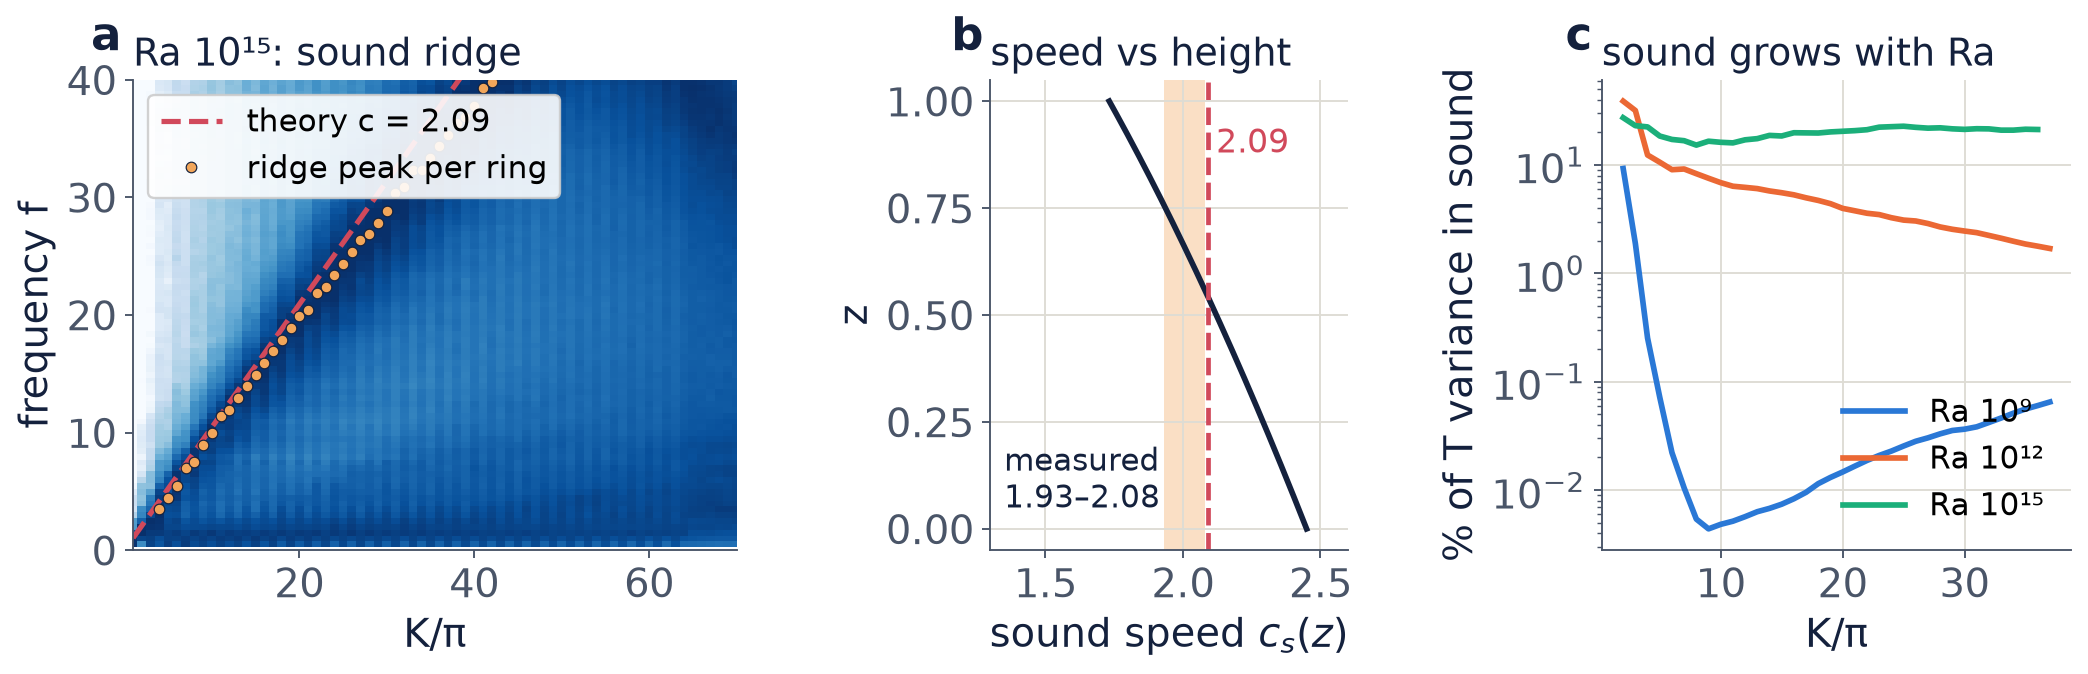
\includegraphics[width=\textwidth]{../figures/report/rep_sound.png}
\caption{Sound waves. (a) Power against size and frequency at $\mathrm{Ra}=10^{15}$ (darker = more power, normalised per ring). Dots: peak frequency of the ridge in each ring; dashed: ideal-gas sound speed, not fitted. (b) Ideal-gas sound speed against height; it falls from 2.45 at the hot bottom to 1.73 at the cold top. The travel-time average is 2.09; the shaded band is the measured range. (c) Share of the temperature variance carried by sound, by size.}\label{fig:sound}
\end{figure}

\textbf{Theory with no fit.} Velocities in the simulation are measured in free-fall units $U=\sqrt{g\,d\,\varepsilon}$. For an ideal gas with the adiabatic background $T_A=1-Dz$, the sound speed in these units is
\[ \frac{c_s(z)}{U} = \sqrt{\frac{(\gamma-1)\,T_A(z)}{D\,\varepsilon}}, \]
which falls from 2.45 at the bottom to 1.73 at the top (Fig.~\ref{fig:sound}b). A wave crossing the depth feels the travel-time average $\bar c=\big[\int_0^1 dz/c_s\big]^{-1}=2.09$. This number uses only $\gamma$, $D$ and $\varepsilon$ printed on the movie.

\textbf{Measurement.} The peak frequency in each ring gives $\omega(K)$, and a straight-line fit through the origin gives $c$ (Table~\ref{tab:sound}). In both the temperature and the density panels, at both high Rayleigh numbers, the measured speed is $1.93$--$2.08$, within 8\% of the theory. The ridge is slightly below the depth-average line in the temperature panel, as expected if the waves are weighted toward the cooler upper half, where the temperature fluctuations are strongest.

\begin{table}[H]\centering\small
\caption{Sound waves from the frequency--wavenumber spectrum. Speed from a line fit to the ridge peaks ($K/\pi=4$--$60$); share = fraction of the variance on the ridge at $K/\pi=10$--$30$.}\label{tab:sound}
\begin{tabular}{@{}lccc@{}}
\toprule
 & \color{blue9}$\mathbf{Ra=10^{9}}$ & \color{org12}$\mathbf{Ra=10^{12}}$ & \color{grn15}$\mathbf{Ra=10^{15}}$\\
\midrule
Ridge speed, temperature panel & no ridge & $1.93$ \scriptsize(37 rings) & $1.93$ \scriptsize(39 rings)\\
Ridge speed, density panel & no ridge & $2.08$ \scriptsize(35 rings) & $2.00$ \scriptsize(34 rings)\\
Ideal-gas theory (no fit) & \multicolumn{3}{c}{$2.09$}\\
Share of $T$ variance in sound & $<0.1\%$ & $4.2\%$ & $20.5\%$\\
Share of $\rho$ variance in sound & $0.1\%$ & $7.2\%$ & $17.2\%$\\
\bottomrule
\end{tabular}
\end{table}

\textbf{Why it matters.} Sound is only about twice as fast as the flow's own speed scale here, so the gas is strongly compressible and the waves mix with the turbulence. Their share grows steeply with Ra (Fig.~\ref{fig:sound}c): none at $10^{9}$, about 4\% at $10^{12}$ and 20\% at $10^{15}$, where they form part of the pressure fluctuations of Section~\ref{sec:entropy}. The 3D movie at $10^{8}$ shows no ridge (below 0.4\%). Together with the steep vortex-core spectrum, sound waves are a likely contributor to the steeper slope at $10^{15}$.

\subsection{The 3D movie}
The 3D movie shows only the outer faces of the box, so a full 3D FFT is not possible; the four drawn walls are only two independent planes, each drawn twice. On the walls the same mirror-trick analysis gives ring slopes of $-2.05$ and $-1.93$ ($K/\pi=5$--$15$) and entropies of 3.83 and 4.33 bits. On the lid and the floor the slopes along $x$ and $y$ agree, so the horizontal planes are isotropic. Every cold spot is also heavy: the cold structures are plumes, with a pressure share of only 7.3\% \scriptsize[6.8, 7.8]\normalsize, against 97\% in 2D at high Ra.

\section{Theory against measurement}
\begin{center}\small
\begin{tabular}{@{}p{5.2cm}p{3.0cm}p{5.6cm}c@{}}
\toprule
\textbf{Test} & \textbf{Theory} & \textbf{Measured} & \textbf{Match}\\
\midrule
Obukhov--Corrsin scalar spectrum & $-5/3$ & $-1.59$ (1D), $-1.62$ (2D) at $10^{12}$ & yes\\
Sharp fronts at small scales & $-2$ & $-1.97$, $-1.92$ & yes\\
$k^{-2}$ branch from the plates & ratio 1, slope $-2$ & $0.98$, $1.00$; $-2.15$, $-2.09$ & yes\\
Ideal-gas constants & $\gamma-1=0.30$, $D=0.50$ & $0.29$, $0.48$ & yes\\
Near-isotropic bulk & $E_z/E_x\approx1$ & $1.01$--$1.17$ & yes\\
Ideal-gas sound speed & $2.09$ & $1.93$--$2.08$ & yes\\
Boussinesq up--down symmetry & jumps $0.5\,\varepsilon$, $0.5\,\varepsilon$ & $0.25\,\varepsilon$, $0.75\,\varepsilon$ & no (compressible)\\
Obukhov--Corrsin at $10^{15}$ & $-5/3$ & $-2.35$ (1D), $-2.27$ (2D) & no (vortex cores)\\
\bottomrule
\end{tabular}\end{center}

\section{Limits and conclusions}
\begin{itemize}[leftmargin=1.2em,itemsep=2pt]
\item \textbf{Movie pixels are enough.} Every test that needs no fitted constant passes: $-5/3$ at $\mathrm{Ra}=10^{12}$, the $k^{-2}$ branch from the plates, the gas constants, bulk isotropy and the sound speed.
\item \textbf{2D convection at high Ra is dominated by vortex cores}, which steepen the spectrum and lower its entropy; in 3D the cold structures are plumes.
\item \textbf{Compressibility is visible} in the unequal plate jumps and in sound waves that carry up to 20\% of the temperature variance.
\item \textbf{Limits.} At $10^{9}$ video compression limits $k\gtrsim80$. The $10^{12}$ movie holds only about four independent time samples, so its intervals are wide. The $10^{15}$ slope matches no single law; vortex cores and sound waves are the likely causes, but we have not proved which.
\end{itemize}

\begin{keybox}
\textbf{Code.} All code is in a Python package with one folder per result (\texttt{geometry}, \texttt{spectrum\_1d}, \texttt{spectrum\_2d}, \texttt{density}, \texttt{entropy}, \texttt{movie\_3d}, \texttt{validation}, \texttt{figures}). Each number in this report maps to one script in the README; \texttt{run\_all.sh} reproduces everything from the movies. Repository: \href{https://github.com/SUVIDGOEL/idc612-p05-convection}{github.com/SUVIDGOEL/idc612-p05-convection}.
\end{keybox}

\begin{thebibliography}{9}\small
\bibitem{verma2018} M.~K. Verma, \emph{Physics of Buoyant Flows: From Instabilities to Turbulence}, World Scientific (2018).
\bibitem{nath2016} D. Nath, A. Pandey, A. Kumar and M.~K. Verma, Near isotropic behavior of turbulent thermal convection, \emph{Phys. Rev. Fluids} \textbf{1}, 064302 (2016).
\bibitem{kumar2018} A. Kumar and M.~K. Verma, Applicability of Taylor's hypothesis in thermally driven turbulence, \emph{R. Soc. Open Sci.} \textbf{5}, 172152 (2018).
\bibitem{verma2022} M.~K. Verma and S. Chatterjee, Hydrodynamic entropy and emergence of order in two-dimensional Euler turbulence, \emph{Phys. Rev. Fluids} \textbf{7}, 114608 (2022).
\bibitem{castaing1989} B. Castaing \emph{et al.}, Scaling of hard thermal turbulence in Rayleigh--Bénard convection, \emph{J. Fluid Mech.} \textbf{204}, 1--30 (1989).
\end{thebibliography}
\end{document}
